\newcommand\version{v2}
\problemname{Kingdom Division}
In a far away kingdom, there are $N$ cities numbered between $0$ and $N - 1$.
The cities are connected by $N - 1$ two-way roads.
Each road connects exactly two cities, such that there is a unique path between any pair of cities. Each city $i$ has some value $C[i]$ (possibly negative).

Unfortunately, the old king of the kingdom died, without appointing a successor. Thus a civil war broke out in the kingdom, between the $P$ lords who wish to gain control of the kongdom.

After a long and terrible war, the lords realized none of them could beat all the other lords in the war. They agreed to a truce, and decided to divide the kingdom into $P$ parts, one part per lord. The parts must be so that if two cities $a$ and $b$ lie in the same part, all cities in the unique path between them must also lie in that part.

Since no lord wants to get less than another, the value of each part must be the same. The value of a part is the sum of the values of all cities in that part.

\section*{Example}
Let the kingdom have $N = 5$ cities, connected by roads as in the figure below:
\begin{figure}[h!]
  \centering
  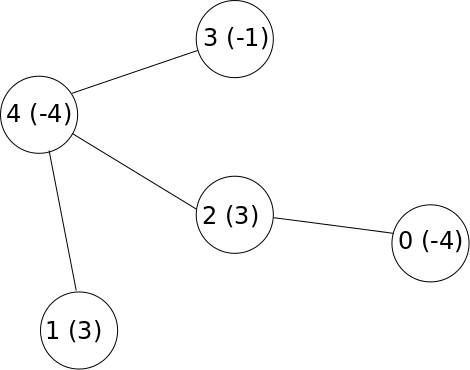
\includegraphics[width=0.3\textwidth]{sample.png}
  \caption{Illustration of the example}
\end{figure}
Each city has its value given within paranthesis after the city number.

In total, we wish to divide the kingdom into $P = 3$ parts.
Then, a possible subdivision would be $(0, 2)$, $(3)$ and $(1, 4)$.
The values of each part would then be $-4 + 3 = -1$, $-1$ and $3 - 4 = -1$,
so all parts in this subdivision would have the same value.

Note that $(0, 1)$, $(3)$, $(2, 4)$ would not be an acceptable division even
though all parts have the same value. This is because the path between cities
$0$ and $1$ is $1, 4, 2, 0$, but cities $4$ and $2$ belong to another part.

\section*{Task}
Your task is to compute a subdivision of the kingdom as described in the statement. You will implement the function \texttt{division(N, P, C, F, T)}.

\begin{itemize}
  \item \texttt{division(N, P, C, F, T)} - this function will be called exactly once by the judge.
  \begin{itemize}
    \item \texttt{N}: the number of cities in the kingdom.
    \item \texttt{P}: the number of parts we wish to divide the kingdom into.
    \item \texttt{C}: an array with $N$ elements. \texttt{C[i]} ($0 \le i < N$) contains the value of city $i$.
    \item \texttt{F}: an array with $N - 1$ elements. \texttt{F[i]} ($0 \le i < N - 1$) contains one of the cities that the $i$:th road connects.
    \item \texttt{T}: an array with $N - 1$ elements. \texttt{T[i]} ($0 \le i < N - 1$) contains the other city that the $i$:th road connects.
    \item It is always possible to travel between any pair of cities using the roads.
		\item $|C[i]| < 10^9$
		\item The function should return 1 if it is possible to find such a subdivision,
			and 0 if it is impossible.
  \end{itemize}
\end{itemize}

Additionally, you should make calls to the function \texttt{part(S, R)} to construct your subdivision.
\begin{itemize}
  \item \texttt{part(S, R)} - this function should be called once for each of the $P$ parts of the subdivision.
  \begin{itemize}
    \item \texttt{S}: the number of cities in the part.
    \item \texttt{R}: an array with $S$ elements - the numbers of the cities in the part.
		\item The function has no return value.
  \end{itemize}
\end{itemize}

\section*{Subtasks}
The problem consists of a number of subtasks. Each subtask gives some amount of points, and to pass
the subtask you must pass all the test cases in the subtask.

If your partition is incorrect, but you correctly determine whether a partition exists, your solution
will get $50\%$ of the score. 
\begin{tabular}{|l|l|l|}
  \hline
  \textbf{Subtask} & \textbf{Points} & \textbf{Limits} \\ \hline
  1 & 8 & $N \le 10, P = 2$ \\ \hline
	2 & 10 & $1 \le P \le N \le 1\,000$, $C[i] > 0$ \\ \hline
	3 & 16 & $1 \le P \le N \le 1\,000$, only cities $i$ and $i + 1$ have roads (for $0 \le i < N - 1$). \\ \hline
  4 & 18 & $1 \le P \le N \le 1\,000$ \\ \hline
	5 & 18 & $1 \le P \le N \le 100\,000$, $C[i] > 0$ \\ \hline
  6 & 30 & $1 \le P \le N \le 100\,000$ \\ \hline
\end{tabular}

\section*{Input format}
The sample judge reads input in the following format:

\begin{itemize}
  \item line $1$: \texttt{N P}
  \item line $2$: \texttt{C[0] C[1] .. C[N - 1]}
  \item line $3$: \texttt{F[0] F[1] .. F[N - 2]}
  \item line $4$: \texttt{T[0] T[1] .. T[N - 2]}
\end{itemize}

\section*{Output format}
The sample judge will first write a single line with the return value of \texttt{paths(N, K, F, T)}. The next line will contain $N$ integers containing the input to the \texttt{parts(R)} call.
